% id: 0360
% book: 쎈 중3-2 수학 · 03 원과 직선
% section: 유형 14 직각삼각형의 내접원
% figure: tikz:fig-0360
% answer: ⑤
% answer_source: 답지
% variant_level: 0 (원본 전사)
% 이 파일은 build.mjs 가 items.json 에서 만든다. 고칠 때는 items.json 을 고친다.
\smash{\raisebox{1.5mm}{\dmkichul{쎈 중3-2 수학 0360번 · 67쪽}}}
\noindent\begin{minipage}[t]{0.58\linewidth}\vspace{0pt}\raggedright 오른쪽 그림과 같이 $\seg{AB}=8\,\mathrm{cm}$, $\seg{BC}=17\,\mathrm{cm}$인 직사각형~$\pt{ABCD}$를 꼭짓점~$\pt{B}$가 $\seg{AD}$ 위의 점~$\pt{E}$에 오도록 $\seg{FC}$를 접는 선으로 하여 접었다. 원~$\pt{O}$는 $\triangle\pt{CDE}$의 내접원이고 세 점~$\pt{G}$, $\pt{H}$, $\pt{I}$는 접점일 때, 원~$\pt{O}$의 반지름의 길이는?\end{minipage}\hfill\begin{minipage}[t]{0.4\linewidth}\vspace{0pt}\centering \resizebox{\ifdim\width>\linewidth\linewidth\else\width\fi}{!}{% 0360(본책 67쪽) — 직사각형 ABCD(AB=8 cm, BC=17 cm)를 FC 로 접어 B 가 AD 위 E 에 옴, △CDE 의 내접원 O(접점 G, H, I), 접힌 △EFC 색칠. 답(반지름)은 적지 않는다. 스캔 삽화를 TikZ 로 다시 그림.
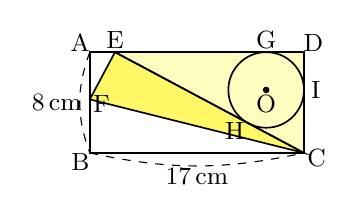
\begin{tikzpicture}[line width=0.6pt]
  \fill[yellow!25] (0.320,1.280) -- (2.720,0.000) -- (2.720,1.280) -- cycle;
  \fill[yellow!60] (0.320,1.280) -- (0.000,0.680) -- (2.720,0.000) -- cycle;
  \draw (0.000,1.280) -- (0.000,0.000) -- (2.720,0.000) -- (2.720,1.280) -- cycle;
  \draw (0.320,1.280) -- (0.000,0.680) -- (2.720,0.000) -- cycle;
  \draw (0.320,1.280) -- (2.720,0.000);
  \draw (2.240,0.800) circle (0.480);
  \fill (2.240,0.800) circle (1.2pt);
  \draw[dashed, line width=0.4pt] (0.000,1.280) to[bend right=20] (0.000,0.000);
  \node[font=\small, inner sep=1.5pt] at (-0.420,0.640) {$8\,\mathrm{cm}$};
  \draw[dashed, line width=0.4pt] (0.000,0.000) to[bend right=12] (2.720,0.000);
  \node[font=\small, inner sep=1.5pt] at (1.360,-0.300) {$17\,\mathrm{cm}$};
  \node[font=\small, inner sep=1.5pt] at (-0.120,1.400) {A};
  \node[font=\small, inner sep=1.5pt] at (-0.120,-0.120) {B};
  \node[font=\small, inner sep=1.5pt] at (2.880,-0.058) {C};
  \node[font=\small, inner sep=1.5pt] at (2.840,1.400) {D};
  \node[font=\small, inner sep=1.5pt] at (0.320,1.430) {E};
  \node[font=\small, inner sep=1.5pt] at (0.150,0.625) {F};
  \node[font=\small, inner sep=1.5pt] at (2.240,1.430) {G};
  \node[font=\small, inner sep=1.5pt] at (1.841,0.276) {H};
  \node[font=\small, inner sep=1.5pt] at (2.870,0.800) {I};
  \node[font=\small, inner sep=1.5pt] at (2.240,0.620) {O};
\end{tikzpicture}
}\end{minipage}\par
\begin{choices32}{$1\,\mathrm{cm}$}{$1.5\,\mathrm{cm}$}{$2\,\mathrm{cm}$}{$2.5\,\mathrm{cm}$}{$3\,\mathrm{cm}$}\end{choices32}
